\documentclass[12 pt]{article}
\usepackage[margin= 1in]{geometry}
\usepackage{amssymb,amsmath}
\usepackage[pdftex]{graphicx}
\usepackage{fourier}

\begin{document}


\newcommand{\boldbeta}{\boldsymbol{\beta}}
\newcommand{\boldy}{\boldsymbol{y}}
\newcommand{\boldX}{\boldsymbol{X}}
\newcommand{\boldx}{\boldsymbol{x}}
\newcommand{\boldz}{\boldsymbol{z}}
\newcommand{\boldgamma}{\boldsymbol{\gamma}}
\newcommand{\boldeps}{\boldsymbol{\epsilon}}


\setlength{\parskip}{1ex plus 0.5ex minus 0.2ex}

\setcounter{secnumdepth}{-2}


\begin{flushleft}
  

Vanderbilt University \\
Leadership, Policy and Organizations \\
Class Number 9553 \\
Spring 2018 \\
\end{flushleft}

\begin{centering}
\textbf{\large{Models for Categorical Outcomes}}  
\end{centering}


\section{Ordered Outcomes}

We many times work with data that is categorical (mutually exclusive and exhaustive
categories), but ordered--- each level implies going up or down from the previous level.
What makes this ordinal data is that the steps do not imply the same distance on a
given scale. For instance, consider an outcome like educational attainment, coded as
less than high school, high school, some college, bachelor's degree, advanced degree.
While these are clearly ordered---each step implies going up the educational ladder---
the distance between steps is not as simple as the number of years of education.
For this situation we can use the ordered probit model. 


\subsection{Econometric Model}
\label{sec:econometric-model}

The random  utiliity form of the ordered probit model is as follows:

\begin{equation*}
  \boldy^*_i=\boldx \boldbeta + e_i, \qquad e_i  \sim N (0,1)   i=1  \ldots N
\end{equation*}


$y_i$, the observed variable takes on values $0$ through $m$:
\begin{equation*}
  y_i=j \iff \tau_{j-1}< y^*_i \leq \tau_{j} 
\end{equation*}

For the ordinal probit model, the assumption is that $e_i$ is
distributed normally with mean 0, and typically standard deviation 1. 

We then will have defined $y^*$ as being within a normal distribution,
with the probability space from 0 to 1 divided by a set of cut point $\tau_k$

The probability that y=1 is given by:

\begin{equation*}
  Pr(y_i=1| \boldx_i)=Pr(\tau_0\leq y_i^* < \tau_1|\boldx)
\end{equation*}

Substituting from above and evaluating the cdf of the normal
distribution ($\phi$) to calculate probabilities within each space
gives use the following. 

To find the probability that $y=m$, we utilize the following equation

\begin{equation*}
  P(y_i=m)=\phi(\tau_m-\boldx_i\boldbeta)-\phi(\tau_{m-1}-\boldx_i\boldbeta)
\end{equation*}

This is actually a generalization of the probit model for binary
response-- in the binary case, m can be 0 or 1, while in the ordered
case, m can take on any number of values. 

This model is not identified without an additional assumption. We can
either set the intercept in the linear model to be constant, usually
at 0,  $(\beta_0=0)$ or we can assume
that $\tau_1$=0. By default, Stata holds $(\beta_0=0)$. 

\subsection{Reporting Results}
\label{sec:reporting-results}

These models can be difficult to interpret for the same reason the
models for binary data can be difficult: the interpretation is on the
logit scale or the normal scale, and parameter estimates cannot be
interpreted one at a time in terms of probability. I present two
options below. 

Consider the following set of results from an ordinal probit
regression of college plans (Don't know=1, Two year=2, Four year=3) on
a set of student characteristics. 

\begin{table}
  \centering
  \caption{Results of Ordinal Probit Estimates, Dependent Variable= College Plans (None, 2yr, 4yr)}
   \begin{footnotesize}
\begin{tabular}{l*{3}{c}}
\hline\hline
            &\multicolumn{1}{c}{(1)}&\multicolumn{1}{c}{(2)}&\multicolumn{1}{c}{(3)}\\
            &\multicolumn{1}{c}{order\_plan}&\multicolumn{1}{c}{order\_plan}&\multicolumn{1}{c}{order\_plan}\\
\hline
order\_plan  &            &            &            \\
female      &        0.29&        0.29&        0.31\\
            &      (0.02)&      (0.02)&      (0.02)\\
[1em]
bynels2m    &        2.52&        2.70&        2.37\\
            &      (0.13)&      (0.13)&      (0.13)\\
[1em]
bynels2r    &        2.66&        2.94&        2.38\\
            &      (0.18)&      (0.19)&      (0.19)\\
[1em]
amind       &            &        0.04&        0.13\\
            &            &      (0.12)&      (0.12)\\
[1em]
asian       &            &        0.35&        0.44\\
            &            &      (0.04)&      (0.04)\\
[1em]
black       &            &        0.48&        0.55\\
            &            &      (0.04)&      (0.04)\\
[1em]
hispanic    &            &        0.05&        0.19\\
            &            &      (0.03)&      (0.03)\\
[1em]
multiracial &            &       -0.00&        0.02\\
            &            &      (0.05)&      (0.05)\\
[1em]
byses1      &            &            &        0.38\\
            &            &            &      (0.02)\\
\hline
cut1        &            &            &            \\
\_cons      &        0.46&        0.70&        0.42\\
            &      (0.04)&      (0.05)&      (0.05)\\
\hline
cut2        &            &            &            \\
\_cons      &        1.68&        1.94&        1.68\\
            &      (0.04)&      (0.05)&      (0.05)\\
\hline
\(N\)       &       13055&       13055&       13055\\
\textit{AIC}&    19165.26&    18947.23&    18493.51\\
\hline\hline
\multicolumn{4}{l}{\footnotesize Standard errors in parentheses}\\
\end{tabular}


  \label{tab:order}
\end{footnotesize}
\end{table}

\clearpage
Without additional interpretation, this doesn't make sense. One way to
interpret results is to use marginal effects, calculated for each
outcome, holding all other variables at their means. 


\begin{table}
  \centering
  \caption{Marginal Effects for Variables, Dependent Variable= College
    Plans (None, 2yr, 4yr) Outcomes in Columns}
   \begin{footnotesize}
\begin{tabular}{l*{3}{c}} \hline\hline
            &\multicolumn{1}{c}{(1)}&\multicolumn{1}{c}{(2)}&\multicolumn{1}{c}{(3)}\\
            &\multicolumn{1}{c}{}  &\multicolumn{1}{c}{}  &\multicolumn{1}{c}{}  \\
\hline
bynels2m    &                 -0.28&                 -0.44&                  0.72\\
            &         [-0.31,-0.25]&         [-0.49,-0.40]&           [0.65,0.80]\\
[1em]
bynels2r    &                 -0.28&                 -0.45&                  0.72\\
            &         [-0.32,-0.23]&         [-0.51,-0.38]&           [0.61,0.83]\\
[1em]
amind       &                 -0.02&                 -0.02&                  0.04\\
            &          [-0.04,0.01]&          [-0.07,0.02]&          [-0.03,0.11]\\
[1em]
asian       &                 -0.05&                 -0.08&                  0.13\\
            &         [-0.06,-0.04]&         [-0.10,-0.07]&           [0.11,0.16]\\
[1em]
black       &                 -0.06&                 -0.10&                  0.17\\
            &         [-0.07,-0.06]&         [-0.12,-0.09]&           [0.15,0.19]\\
[1em]
hispanic    &                 -0.02&                 -0.04&                  0.06\\
            &         [-0.03,-0.01]&         [-0.05,-0.02]&           [0.04,0.08]\\
[1em]
multiracial &                 -0.00&                 -0.00&                  0.01\\
            &          [-0.02,0.01]&          [-0.02,0.02]&          [-0.03,0.04]\\
[1em]
byses1      &                 -0.04&                 -0.07&                  0.12\\
            &         [-0.05,-0.04]&         [-0.08,-0.06]&           [0.11,0.13]\\
\hline
\(N\)       &                 13055&                 13055&                 13055\\
\hline\hline
\multicolumn{4}{l}{\footnotesize 95\% confidence intervals in brackets}\\
\end{tabular}


  \label{tab:order_marg}
\end{footnotesize}
\end{table}

\clearpage


As always, I reccomend plotting the data. The figure below shows the predicted
impact of test scores on the probability of each outcome, holding all
other variables constant at their minimum for binary variables and at
their mean for continuous variables.

\begin{figure}
  \centering
  
  \caption{Predicted Impact of Math Test Scores on College Plans,
    Outcome= Don't Know, Two Year College, Four Year College}
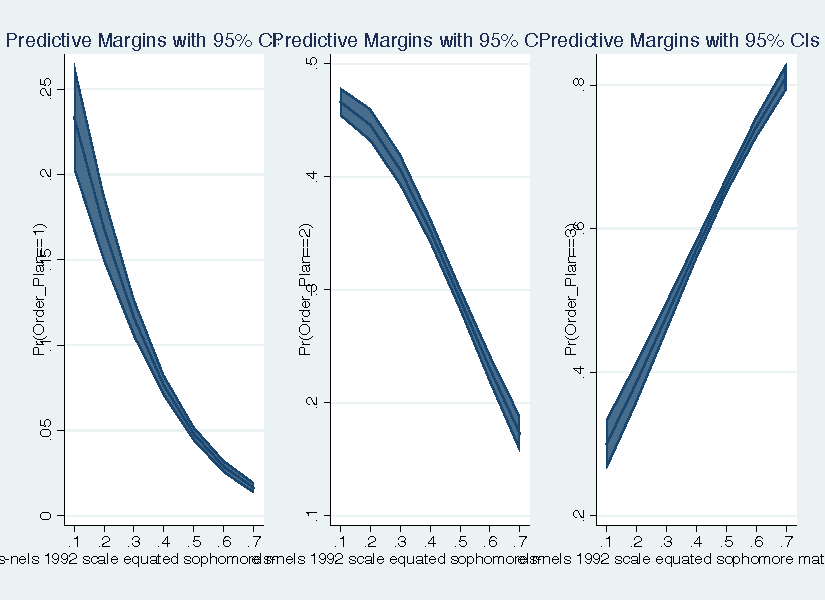
\includegraphics[width=\textwidth]{order}
  \label{fig:order}
\end{figure}

\clearpage

\subsection{Quick Exercise}
\label{sec:quick-exercise}

Conduct a regression with institution of first attendance as an ordered outcome
and report on the results. 


\section{ Unordered Outcomes}
When dealing with unordered categorical data, we no longer have the information that
the outcomes share some agreed order. Instead, we have categorical information. A
classic example is the type of college a student attends: public four year, private four
year, public two year. The choices are not ordered in any way that makes sense.
The model here is more complicated. We need to model tradeoffs between each of
the choices. The model here takes the form:
\begin{align*}
  Pr(Y_i=1) & =Pr(\mu_{i1}>\mu_{i2})  \\
&=Pr( \mu_{i1} + e_{i1}  > \mu_{i2}+ e_{i2} )  \\
& = Pr( e_{i1} - e_{i2} > \mu_{i2} - \mu_{i1}  ) 
\end{align*}

In effect, we are comparing each of the choices with one another,
with utility set, as always, to = $\boldx \boldbeta$

\begin{equation*}
  Pr(y=m)=Pr(\boldx \boldbeta_m > \boldx \boldbeta_j  \forall  j
  \neq m)
\end{equation*}

This means that all coefficients will be \emph{relative}. Below are
the coefficients for a model of first instiitution attended, with
public two year, other and private four year compared to public four year. 


\begin{table}
  \centering
  \caption{Results of Multinomial Logit model, outcome= First College
    Attended}
   \begin{tiny}
{
\def\sym#1{\ifmmode^{#1}\else\(^{#1}\)\fi}
\begin{tabular}{l*{3}{c}}
\hline\hline
            &\multicolumn{1}{c}{(1)}&\multicolumn{1}{c}{(2)}&\multicolumn{1}{c}{(3)}\\
            &\multicolumn{1}{c}{first\_inst}&\multicolumn{1}{c}{first\_inst}&\multicolumn{1}{c}{first\_inst}\\
\hline
Public\_4\_Year&                     &                     &                     \\
female      &        0.00         &        0.00         &        0.00         \\
            &         (.)         &         (.)         &         (.)         \\
[1em]
bynels2m    &        0.00         &        0.00         &        0.00         \\
            &         (.)         &         (.)         &         (.)         \\
[1em]
bynels2r    &        0.00         &        0.00         &        0.00         \\
            &         (.)         &         (.)         &         (.)         \\
[1em]
amind       &                     &        0.00         &        0.00         \\
            &                     &         (.)         &         (.)         \\
[1em]
asian       &                     &        0.00         &        0.00         \\
            &                     &         (.)         &         (.)         \\
[1em]
black       &                     &        0.00         &        0.00         \\
            &                     &         (.)         &         (.)         \\
[1em]
hispanic    &                     &        0.00         &        0.00         \\
            &                     &         (.)         &         (.)         \\
[1em]
multiracial &                     &        0.00         &        0.00         \\
            &                     &         (.)         &         (.)         \\
[1em]
byses1      &                     &                     &        0.00         \\
            &                     &                     &         (.)         \\
[1em]
\_cons      &        0.00         &        0.00         &        0.00         \\
            &         (.)         &         (.)         &         (.)         \\
\hline
Private\_4\_Year&                     &                     &                     \\
female      &        0.04         &        0.04         &        0.06         \\
            &      (0.06)         &      (0.06)         &      (0.06)         \\
[1em]
bynels2m    &        0.31         &        0.50         &        0.15         \\
            &      (0.33)         &      (0.35)         &      (0.35)         \\
[1em]
bynels2r    &        2.72\sym{***}&        2.39\sym{***}&        1.88\sym{***}\\
            &      (0.47)         &      (0.47)         &      (0.48)         \\
[1em]
amind       &                     &        0.34         &        0.44         \\
            &                     &      (0.41)         &      (0.41)         \\
[1em]
asian       &                     &       -0.39\sym{***}&       -0.34\sym{***}\\
            &                     &      (0.09)         &      (0.09)         \\
[1em]
black       &                     &       -0.05         &        0.02         \\
            &                     &      (0.10)         &      (0.10)         \\
[1em]
hispanic    &                     &       -0.16         &       -0.07         \\
            &                     &      (0.11)         &      (0.11)         \\
[1em]
multiracial &                     &        0.13         &        0.15         \\
            &                     &      (0.13)         &      (0.13)         \\
[1em]
byses1      &                     &                     &        0.36\sym{***}\\
            &                     &                     &      (0.04)         \\
[1em]
\_cons      &       -1.81\sym{***}&       -1.75\sym{***}&       -1.57\sym{***}\\
            &      (0.16)         &      (0.17)         &      (0.17)         \\
\hline
Public\_2\_Year&                     &                     &                     \\
female      &       -0.17\sym{***}&       -0.18\sym{***}&       -0.22\sym{***}\\
            &      (0.05)         &      (0.05)         &      (0.05)         \\
[1em]
bynels2m    &       -4.92\sym{***}&       -5.22\sym{***}&       -4.94\sym{***}\\
            &      (0.29)         &      (0.30)         &      (0.31)         \\
[1em]
bynels2r    &       -4.38\sym{***}&       -4.66\sym{***}&       -4.02\sym{***}\\
            &      (0.40)         &      (0.41)         &      (0.42)         \\
[1em]
amind       &                     &        0.10         &       -0.04         \\
            &                     &      (0.35)         &      (0.35)         \\
[1em]
asian       &                     &       -0.22\sym{**} &       -0.35\sym{***}\\
            &                     &      (0.08)         &      (0.09)         \\
[1em]
black       &                     &       -0.70\sym{***}&       -0.83\sym{***}\\
            &                     &      (0.09)         &      (0.09)         \\
[1em]
hispanic    &                     &        0.21\sym{*}  &        0.04         \\
            &                     &      (0.08)         &      (0.08)         \\
[1em]
multiracial &                     &        0.01         &       -0.01         \\
            &                     &      (0.13)         &      (0.13)         \\
[1em]
byses1      &                     &                     &       -0.46\sym{***}\\
            &                     &                     &      (0.04)         \\
[1em]
\_cons      &        3.64\sym{***}&        3.96\sym{***}&        3.76\sym{***}\\
            &      (0.12)         &      (0.14)         &      (0.14)         \\
\hline
Other       &                     &                     &                     \\
female      &       -0.29\sym{**} &       -0.29\sym{**} &       -0.36\sym{***}\\
            &      (0.09)         &      (0.09)         &      (0.09)         \\
[1em]
bynels2m    &       -7.85\sym{***}&       -7.63\sym{***}&       -7.25\sym{***}\\
            &      (0.51)         &      (0.53)         &      (0.53)         \\
[1em]
bynels2r    &       -3.60\sym{***}&       -3.97\sym{***}&       -3.04\sym{***}\\
            &      (0.71)         &      (0.72)         &      (0.73)         \\
[1em]
amind       &                     &        0.49         &        0.25         \\
            &                     &      (0.48)         &      (0.49)         \\
[1em]
asian       &                     &       -0.65\sym{***}&       -0.88\sym{***}\\
            &                     &      (0.18)         &      (0.19)         \\
[1em]
black       &                     &       -0.27\sym{*}  &       -0.47\sym{***}\\
            &                     &      (0.13)         &      (0.13)         \\
[1em]
hispanic    &                     &        0.39\sym{**} &        0.10         \\
            &                     &      (0.13)         &      (0.13)         \\
[1em]
multiracial &                     &        0.25         &        0.22         \\
            &                     &      (0.21)         &      (0.21)         \\
[1em]
byses1      &                     &                     &       -0.72\sym{***}\\
            &                     &                     &      (0.07)         \\
[1em]
\_cons      &        3.10\sym{***}&        3.14\sym{***}&        2.85\sym{***}\\
            &      (0.18)         &      (0.21)         &      (0.22)         \\
\hline
\(N\)       &        9999         &        9999         &        9999         \\
\textit{AIC}&    22512.33         &    22395.40         &    22039.00         \\
\hline\hline
\multicolumn{4}{l}{\footnotesize Standard errors in parentheses}\\
\multicolumn{4}{l}{\footnotesize \sym{*} \(p<0.05\), \sym{**} \(p<0.01\), \sym{***} \(p<0.001\)}\\
\end{tabular}
}

  \label{tab:multi_results}
\end{tiny}
\end{table}

%                 
\clearpage


\subsection{Quick Exercise}
\label{sec:quick-exercise}

Conduct a regression with a three-part definition of first institution
and report on the results. 


\begin{figure}
  \centering
  
  \caption{Predicted Impact of Math Test Scores on First Institution Attended
    Outcome=Public 4 Year, Private 4 Year, Public 2 Year, Other}
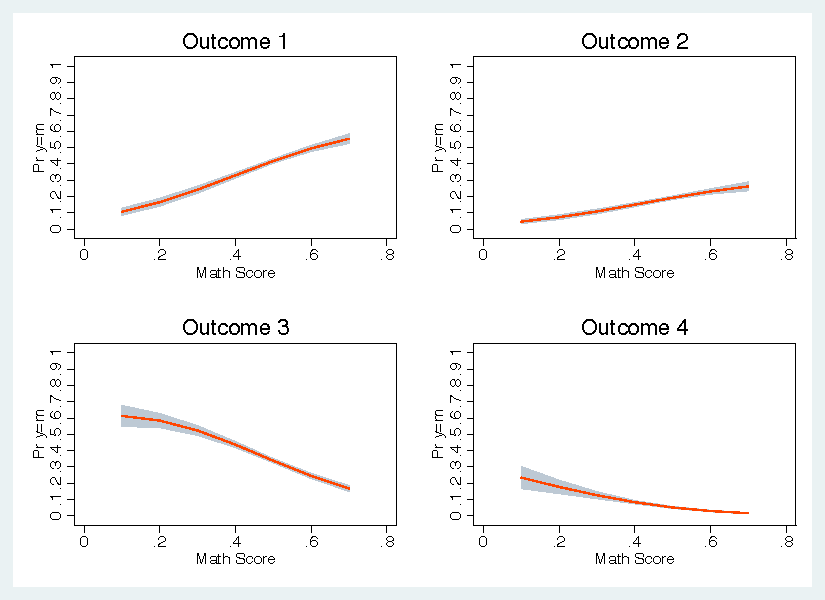
\includegraphics[width=\textwidth]{unorder_first}
  \label{fig:unorder_first}
\end{figure}

As with ordered outcome, the key to interpreting results for a
multinomial model is to predict probabilites and compare those
predicted probabilities.  As we'll see in the case of first
institution choice, the same prospective students will have very
different predicted probabilities of attendance at different types of
institutions. 

Measuring model fit for models for ordered outcomes is almost always
done using the log likelihood. One can use the likelihood ratio test,
AIC or BIC to summarize model fit. There are ways to implement the AUC
for a multiclass outcome, but, it's complicated. 

\end{document}

%%% Local Variables: 
%%% mode: latex
%%% TeX-master: t
%%% End: 
